\documentclass[frenchb]{beamer}
\usepackage[utf8x]{inputenc}
\usepackage[T1]{fontenc}
\usepackage{babel}
\usepackage{listings}
\usepackage{verbatim}
\usepackage{fancyvrb}
\usepackage{color}

	
\setbeamercolor{haut}{fg=white,bg=darkgray}
\setbeamercolor{bas}{fg=black,bg=blue!5}
\lstset{% general command to set parameter(s)
basicstyle=\small,
% print whole listing small
keywordstyle=\color{green},
% underlined bold black keywords
identifierstyle=\color{darkgray},
% nothing happens
commentstyle=\color{white}, % white comments
stringstyle=\ttfamily,
% typewriter type for strings
showstringspaces=false}
% no special string spaces
	
%\usetheme{CambridgeUS}
%\usetheme{Hannover}
\usetheme{Singapore}	
	
\title[M2GL-VET]{Simulateur de synthétiseur de son analogique}
\author{Maxime Simon, Julien Richard-Foy, Julien Névo \& Cyrille Folliot}
\institute[ISTIC]{Université de Rennes 1}
\begin{document}

\begin{frame}
    \titlepage
\end{frame}
	
	
\begin{frame}{Plan de l'intervention}
    \tableofcontents
\end{frame}

\begin{frame}{Présentation du projet}
\end{frame}

\begin{frame}{Un objectif}
    \begin{figure}
        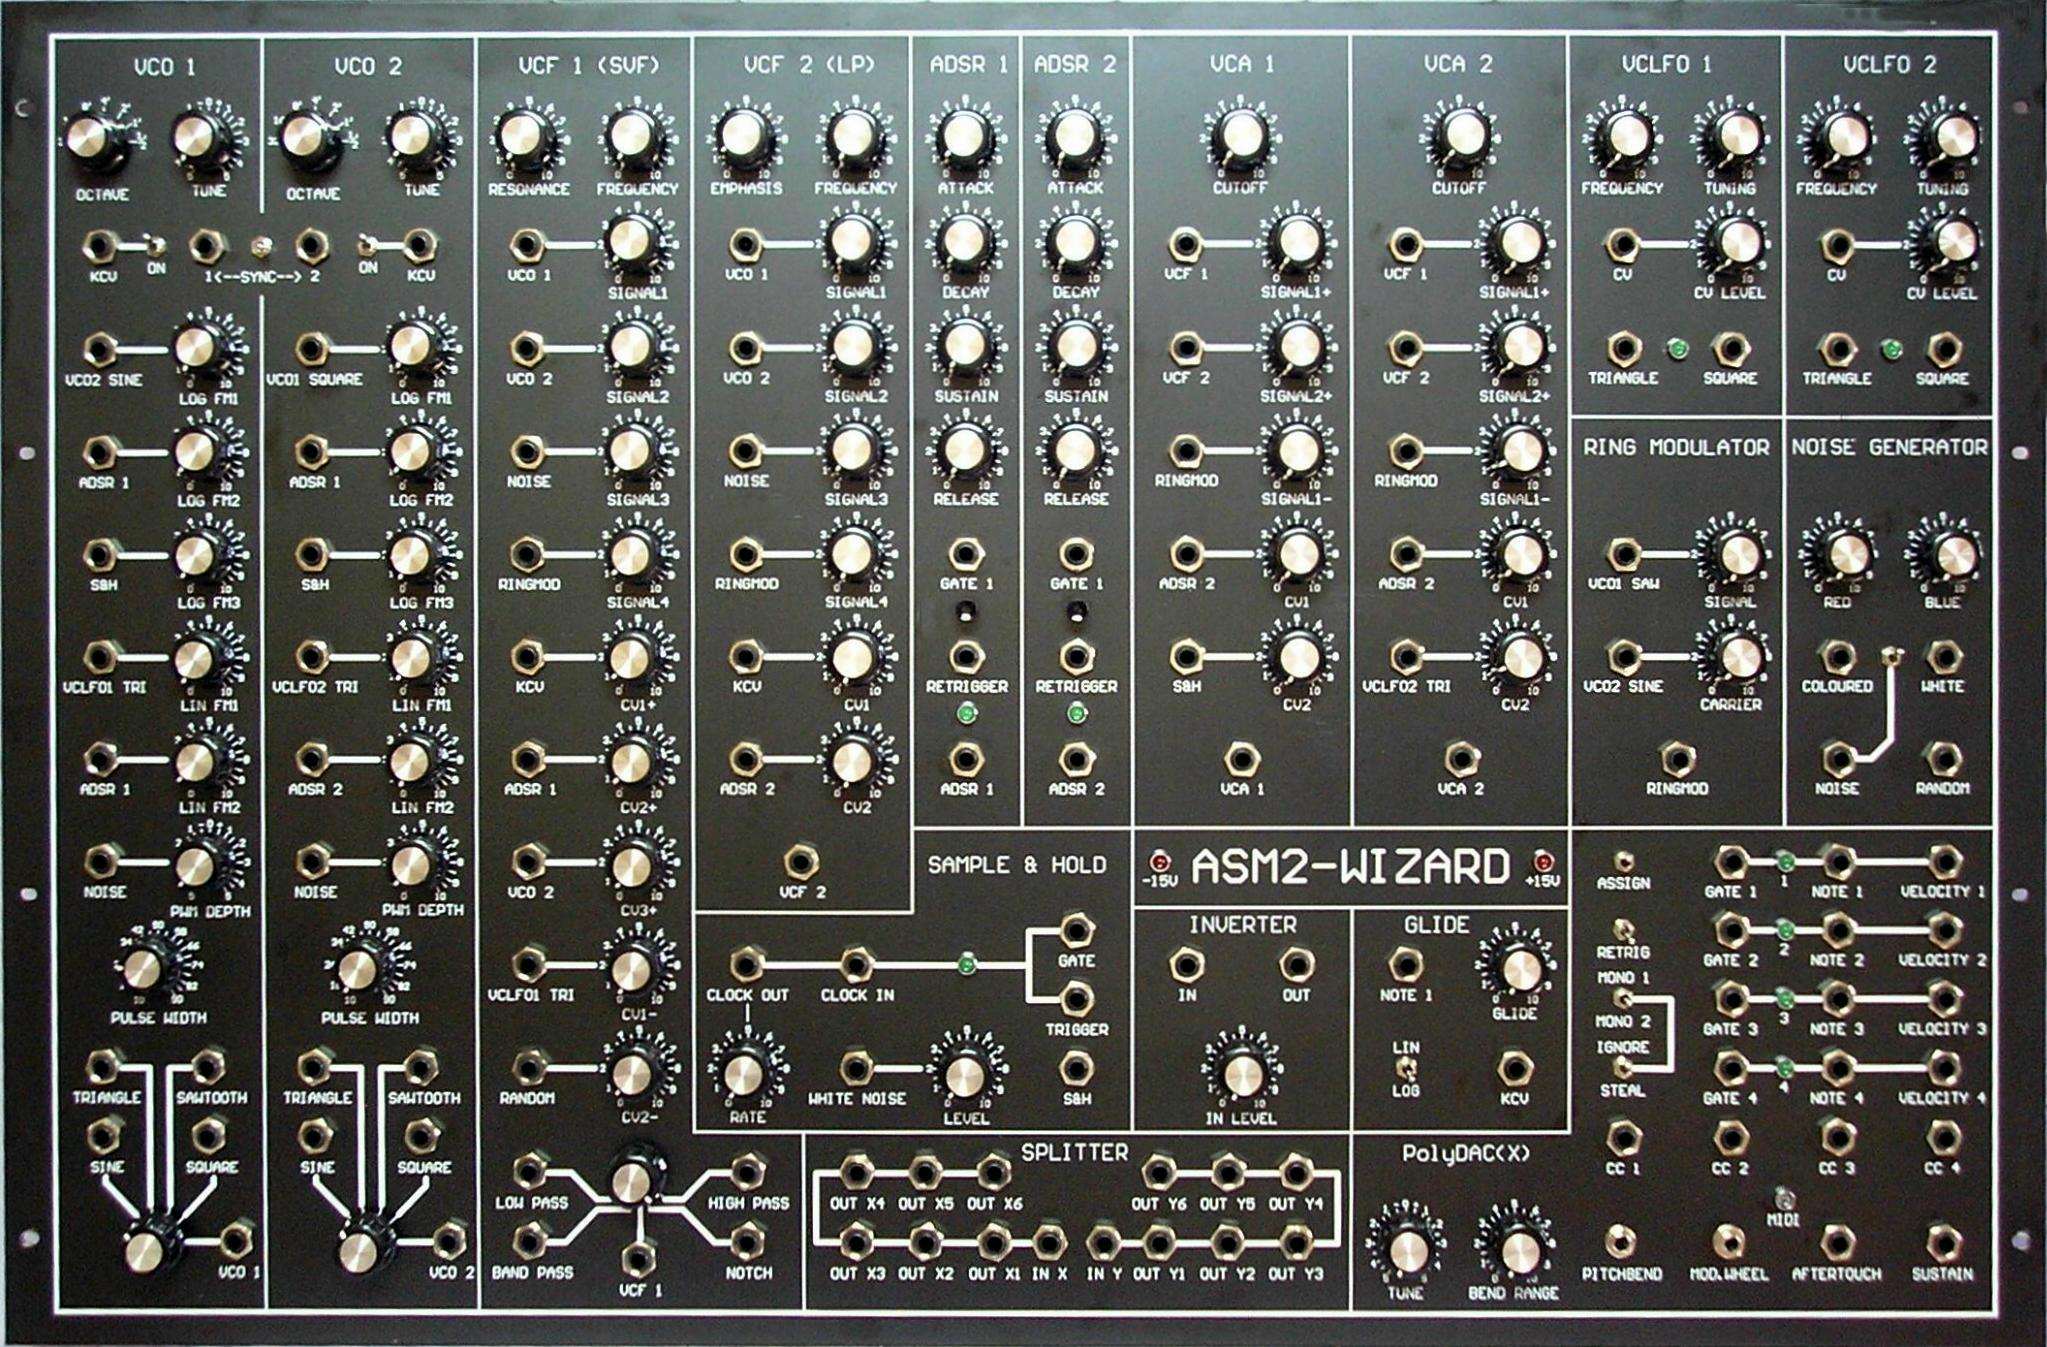
\includegraphics[width=8cm ]{../img/png/synth.jpg}
    \end{figure}
\end{frame}
\begin{frame}{Une équipe}
    \begin{figure}
        
\includegraphics[width=8cm ]{../img/png/back.jpg}
    \end{figure}
\end{frame}

\begin{frame}{L'équipe}
\begin{itemize}    \item Julien Névo~: Responsable projet
    \item Julien Richard-Foy~: Responsable conception
    \item Maxime Simon~: Responsable tests
    \item Cyrille Folliot~: Responsable documentation
\end{itemize}
\end{frame}

\begin{frame}{Organisation du travail}
Le projet comportant deux parties que nous avons distingué lors de l'étude de conception~:
\begin{itemize}
    \item La partie métier (Moteur audio et module du synthétiseur)~: Julien \& Cyrille
    \item L'interface homme-machine~: Maxime \& Julien   
\end{itemize}
\end{frame}

\begin{frame}{Conception - PIM -- Abstraction}
L'architecture de l'abstraction, c'est à dire de la couche métier :
    \begin{figure}
        \includegraphics[width=11cm ]{../img/ps/pim-abstraction.pdf}
    \end{figure}


\end{frame}
Présentation du projet (JN)
Membres de l'équipe
Partage des tâches
Conception (JRF, M)
Tests (C)
Demo (M)
Conclusion (JN)
Retour de l'expérience


\end{document}
